\documentclass[landscape]{article}
% For rotating figures, tables, etc.
%  including their captions
\usepackage[margin=1in]{geometry}

\usepackage{tikz}
\usepackage{tcolorbox}
\usepackage{setspace}
\usepackage{ragged2e}
\usepackage{overpic}

% --- Tikz stuff
\usetikzlibrary{shapes.geometric, hobby, decorations.pathreplacing, calc}
\usetikzlibrary{arrows, arrows.meta}

\definecolor{sapphire}{HTML}{0F52BA}
\definecolor{emerald}{HTML}{27AE60} % 229954} % 50C878}

\begin{document}
\begin{minipage}{.6\textwidth}
    \begin{tikzpicture}[scale=1]
        \node(upper) at (-1, 1){
            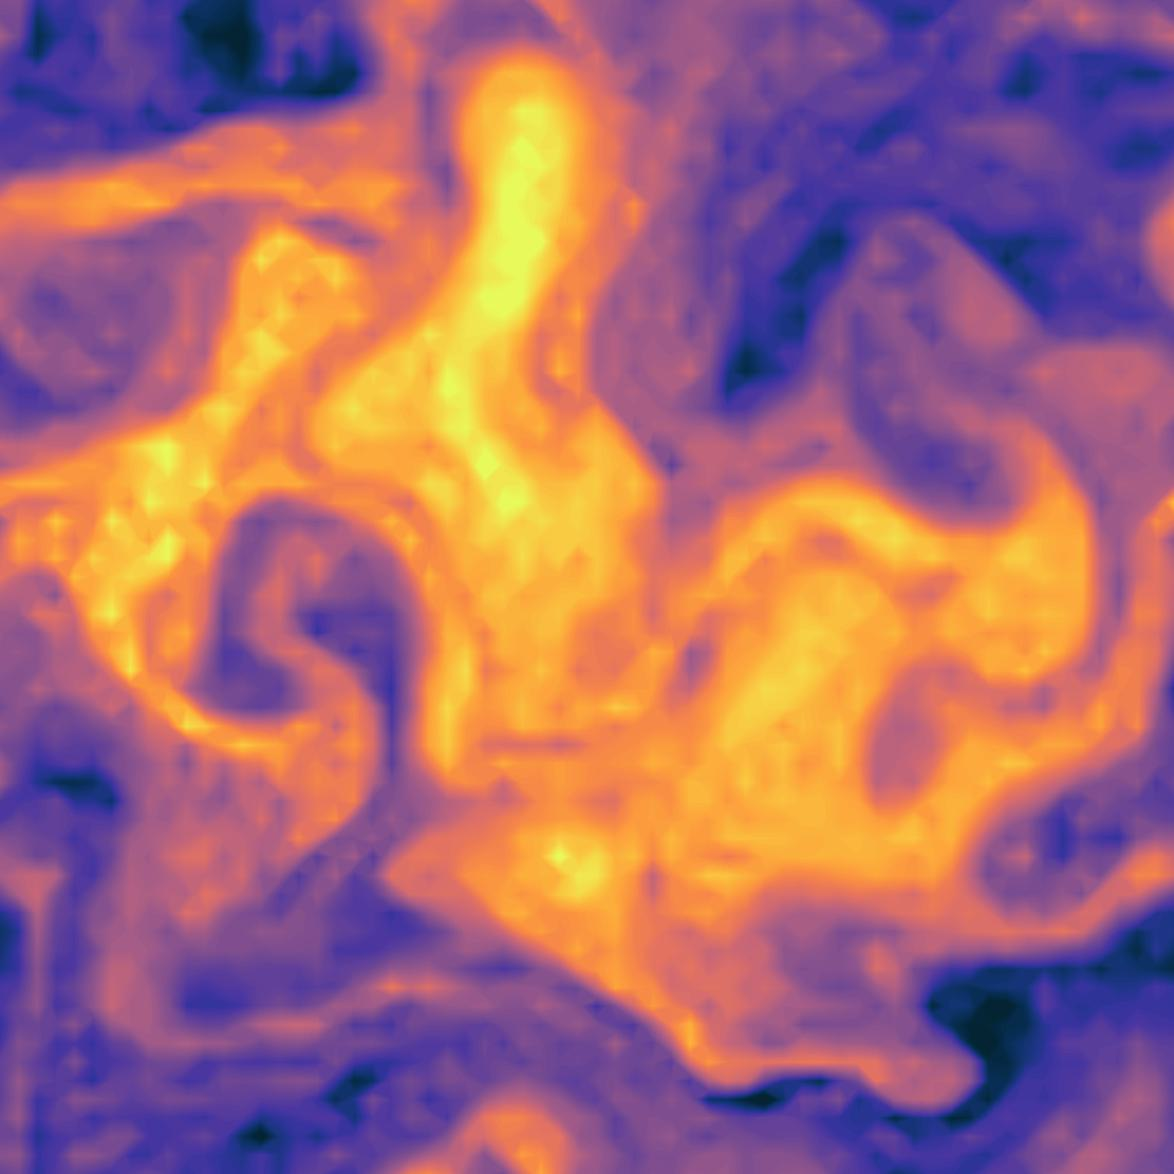
\includegraphics[width=.74\textwidth]{../figures/theta-z1.jpg}
        };
        \node(lower) at (1, -1){
            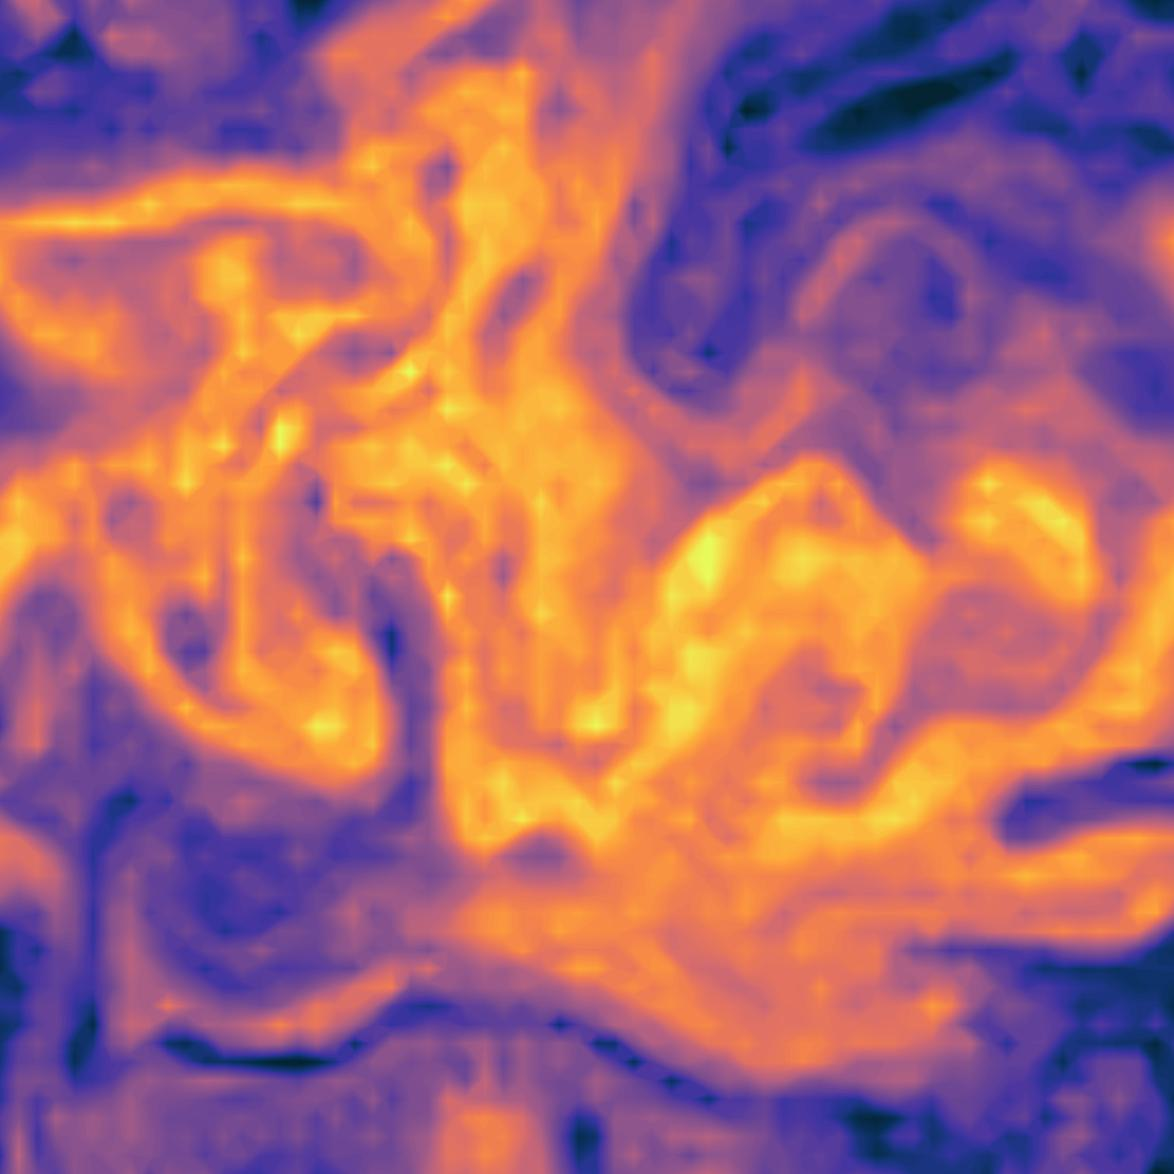
\includegraphics[width=.74\textwidth]{../figures/theta-z0.jpg}
        };
        \draw [line width=5pt,
            {Stealth}-{Stealth}]
            ($ (lower.south west) + (0.45, -0.5) $)
            --
            ($ (lower.south east) - (0.45, 0.5) $)
            node [midway, yshift=-2em] {\Huge $N_x = 64$};
        \draw [line width=5pt,
            {Stealth}-{Stealth}]
            ($ (upper.south west) + (-0.5, 0.45) $)
            --
            ($ (upper.north west) - (0.5, 0.45) $)
            node [midway, xshift=-2em, rotate=90] {\Huge $N_y = 64$};
        \draw [line width=5pt,
            {Stealth}-{Stealth}]
            ($ (upper.south west) - (0.5, 0.5) $)
            --
            ($ (lower.south west) - (0.5, 0.5) $)
            node [midway, xshift=-2em, yshift=-2em, rotate=-45] {\Huge $N_z = 2$};
    \end{tikzpicture}
\end{minipage}

\end{document}
